\documentclass{standalone}
\usepackage{pgfplots}
\usepgfplotslibrary{groupplots}
\pgfplotsset{compat=1.18}
\usepgfplotslibrary{statistics, units}
\usepgflibrary{plotmarks, patterns}
\usetikzlibrary{calc, patterns}
\usepackage{xcolor}
\usepackage{pifont}
\newcommand{\cmark}{\ding{51}}  
\newcommand{\xmark}{\ding{55}}

\definecolor{ibm1}{HTML}{0077BB}
\definecolor{ibm2}{HTML}{33BBEE}
\definecolor{ibm3}{HTML}{EE7733}
\definecolor{ibm4}{HTML}{EE3377}
\definecolor{ibm5}{HTML}{CC3311}


\begin{document}

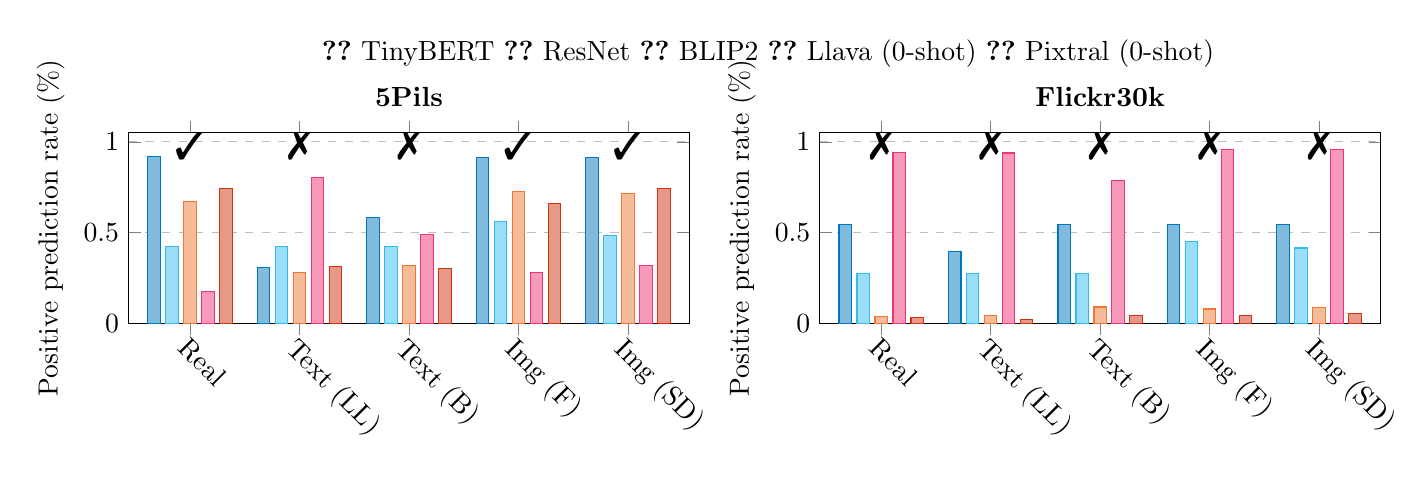
\begin{tikzpicture}
    \begin{groupplot}[
        group style={
            group name=my plots,
            group size=2 by 1,
            horizontal sep=1.66cm
        },
        ybar=2pt,
        /pgf/bar width=4.5pt,
        enlargelimits=0.15,
        enlarge y limits=0,
        scaled y ticks=false, 
        yticklabel style={/pgf/number format/.cd, fixed, precision=2},
        ylabel={Positive prediction rate (\%)},
        width=8.7cm,
        ymax=1.05,
        x tick label style={rotate=-45, anchor=north west, inner sep=0mm},
        symbolic x coords={None, Text (LL), Text (B), Img (F), Img (SD)},
        xtick={None, Text (LL), Text (B), Img (F), Img (SD)},
        xticklabels={Real, Text (LL), Text (B), Img (F), Img (SD)},
        legend columns=3,
        height=4cm,
        ymajorgrids=true,
        grid style=dashed,
        ymin=0,
        enlarge x limits=0.14,
        nodes near coords align={vertical},
        legend image code/.code={%
            \draw[#1] (0cm,-0.1cm) rectangle (0.6cm,0.1cm);
        }
    ]

    % postaction={pattern=north east lines},
    \nextgroupplot[title=\textbf{5Pils}]
        \addplot[fill=ibm1!50, draw=ibm1] coordinates {(None,0.9181636726546906) (Text (LL),0.30538922155688625) (Text (B),0.5808383233532934) (Img (F),0.916) (Img (SD),0.914)};
        \label{plot:series1}
        \addplot[fill=ibm2!50, draw=ibm2] coordinates {(None,0.423) (Text (LL),0.423) (Text (B),0.423) (Img (F),0.560) (Img (SD),0.482)};
        \label{plot:series2}
        \addplot[fill=ibm3!50, draw=ibm3] coordinates {(None,0.67065868263473) (Text (LL),0.27944111776447106) (Text (B),0.3193612774451098) (Img (F),0.724) (Img (SD),0.713)};
        \label{plot:series3}
        \addplot[fill=ibm4!50, draw=ibm4] coordinates {(None,0.17564870259481039) (Text (LL),0.802) (Text (B),0.4879032258064516) (Img (F),0.28) (Img (SD),0.319672131147541)};
        \label{plot:series4}
        \addplot[fill=ibm5!50, draw=ibm5] coordinates {(None,0.7445109780439122) (Text (LL),0.312) (Text (B),0.3004032258064516) (Img (F),0.66) (Img (SD),0.7438524590163934)};
        \label{plot:series5}
        \coordinate (legend) at (rel axis cs:1,1.38); 
        \node[] at (axis cs:None,           0.98) {\Large \cmark};
        \node[] at (axis cs:{Text (LL)},    0.98) {\Large \xmark};
        \node[] at (axis cs:{Text (B)},     0.98) {\Large \xmark};
        \node[] at (axis cs:{Img (F)},      0.98) {\Large \cmark};
        \node[] at (axis cs:{Img (SD)},     0.98) {\Large \cmark};
        
    \nextgroupplot[title=\textbf{Flickr30k}]
        \addplot[fill=ibm1!50, draw=ibm1] coordinates {(None,0.5452685421994885) (Text (LL),0.3943734015345269) (Text (B),0.5457800511508951) (Img (F),0.5452685421994885) (Img (SD),0.545)};
        \addplot[fill=ibm2!50, draw=ibm2] coordinates {(None,0.2751918158567775) (Text (LL),0.2751918158567775) (Text (B),0.2751918158567775) (Img (F),0.451150895140665) (Img (SD),0.415)};
        \addplot[fill=ibm3!50, draw=ibm3] coordinates {(None,0.03682864450127877) (Text (LL),0.043989769820971865) (Text (B),0.08951406649616368) (Img (F),0.0782608695652174) (Img (SD),0.0859)};
        \addplot[fill=ibm4!50, draw=ibm4] coordinates {(None,0.9432225063938618) (Text (LL),0.9385560675883257) (Text (B),0.7892283790781979) (Img (F),0.9601023017902813) (Img (SD),0.9580562659846548)};
        \addplot[fill=ibm5!50, draw=ibm5] coordinates {(None,0.031713554987212275) (Text (LL),0.01945724526369688) (Text (B),0.041429311237700675) (Img (F),0.043478260869565216) (Img (SD),0.05421994884910486)};
        \node[] at (axis cs:None,           0.98) {\Large \xmark};
        \node[] at (axis cs:{Text (LL)},    0.98) {\Large \xmark};
        \node[] at (axis cs:{Text (B)},     0.98) {\Large \xmark};
        \node[] at (axis cs:{Img (F)},      0.98) {\Large \xmark};
        \node[] at (axis cs:{Img (SD)},     0.98) {\Large \xmark};

    \end{groupplot}

    % Legend outside the plots
    \node at (legend) [anchor=base, xshift=1cm, yshift=0cm] {
        \begin{tabular}{l}
            \ref{plot:series1} TinyBERT 
            \ref{plot:series2} ResNet
            \ref{plot:series3} BLIP2
            \ref{plot:series4} Llava (0-shot)
            \ref{plot:series5} Pixtral (0-shot)
        \end{tabular}
    };

\end{tikzpicture}

\end{document}
